% Pengaturan ukuran teks dan bentuk halaman dua sisi
\documentclass[10pt, twoside]{report}

% Pengaturan ukuran halaman dan margin
\usepackage[a5paper,top=25mm,left=25mm,right=20mm,bottom=25mm]{geometry}

% Pengaturan ukuran spasi
\usepackage[singlespacing]{setspace}

% Judul dokumen
\title{Buku Laporan Kerja Praktek ITC}

% Pengaturan format bahasa
\usepackage[indonesian]{babel}

% Pengaturan detail pada file PDF
\usepackage[pdfauthor={Elon Musk},bookmarksnumbered,pdfborder={0 0 0}]{hyperref}

% Pengaturan jenis karakter
\usepackage[utf8]{inputenc}

% Package lainnya
\usepackage{etoolbox} % Mengubah fungsi default
\usepackage{enumitem} % Pembuatan list
\usepackage{lipsum} % Pembuatan template kalimat
\usepackage{titlesec} % Format judul section
\usepackage{graphicx} % Input gambar
\usepackage{longtable} % Pembuatan tabel
\usepackage[table,xcdraw]{xcolor} % Pewarnaan tabel
\usepackage{natbib} % kutipan artikel

% Definisi untuk "Hati ini sengaja dikosongkan"
\def\kosong{
	\vspace*{\fill}
	\begin{center}\textit{Halaman ini sengaja dikosongkan}\end{center}
	\vfill
}
\patchcmd{\cleardoublepage}{\hbox{}}{\kosong}{}{}

% Pengaturan penomoran halaman
\usepackage{fancyhdr}
\fancyhf{}
\renewcommand{\headrulewidth}{0pt}
\pagestyle{fancy}
\fancyfoot[CE,CO]{\thepage}
\patchcmd{\chapter}{plain}{fancy}{}{}
\patchcmd{\chapter}{empty}{plain}{}{}

% Pengaturan format judul bab
\titleformat{\chapter}[display]{\bfseries\Large}{BAB \centering\Roman{chapter}}{0ex}{\vspace{0ex}\centering}[\vspace{2ex}]
\titleformat{\section}{\bfseries\large}{\MakeUppercase{\thesection}}{1ex}{}
\titleformat{\subsection}{\bfseries\large}{\MakeUppercase{\thesubsection}}{1ex}{}
\titleformat{\subsubsection}{\bfseries\large}{\MakeUppercase{\thesubsubsection}}{1ex}{}
\titlespacing*{\chapter}{0ex}{0ex}{0ex}
\titlespacing{\section}{0ex}{1ex}{1ex}
\titlespacing{\subsection}{0ex}{0.5ex}{0.5ex}
\titlespacing{\subsubsection}{0ex}{0ex}{0ex}

% Pengaturan persamaan
\newenvironment{conditions}
{\par\vspace{\abovedisplayskip}\noindent
	\tabularx{\columnwidth}{>{$}l<{$} @{${}={}$} >{\raggedright\arraybackslash}X}}
{\endtabularx\par\vspace{\belowdisplayskip}}

% Isi keseluruhan dokumen
\begin{document}

  % Nomor halaman pembuka dimulai dari sini
  \pagenumbering{roman}

  % Lembar pengesahaan untuk departemen
  \begin{center}
  {\Large \textbf{LEMBAR PENGESAHAN}}
  \vspace{6ex}

  \addcontentsline{toc}{chapter}{LEMBAR PENGESAHAN (DEPARTEMEN)}

  % Ubah kalimat berikut sesuai dengan judul topik kerja praktik
  {\large \textbf{PEMBUATAN ROKET LUAR ANGKASA ANTI GRAVITASI UNTUK PT. NASA}}
  \vspace{6ex}

  % Ubah kalimat berikut sesuai dengan kalimat pengesahan yang ditentukan oleh departemen
  Laporan Kerja Praktik ini disusun untuk \lipsum[1][1]
  \vspace{2ex}

  % Ubah kalimat-kalimat berikut sesuai dengan tempat dan tanggal pengesahan
  Tempat Pengesahan di: Surabaya \\
  Tanggal: 03 Februari 2021
  \vspace{8ex}

  Menyetujui, \\
  Dosen Pembimbing,
  \vspace{12ex}

  % Ubah kalimat-kalimat berikut sesuai dengan nama dan NIP dosen pembimbing
  \textbf{\underline{Nikola Tesla, S.T., M.T.}} \\
  NIP. 18560710 194301 1 001
  \vspace{8ex}

  Mengetahui, \\
  % Ubah kalimat berikut sesuai dengan jabatan kepala departemen
  Kepala Departemen Teknik Dirgantara FTD - ITS,
  \vspace{12ex}

  % Ubah kalimat-kalimat berikut sesuai dengan nama dan NIP kepala departemen
  \textbf{\underline{Dr. Leonardo Da Vinci, S.T., M.T.}} \\
  NIP 14520415 151905 1 001

\end{center}

  \cleardoublepage

  % Lembar pengesahan untuk perusahaan
  \begin{center}
  {\Large \textbf{LEMBAR PENGESAHAN}}
  \vspace{6ex}

  \addcontentsline{toc}{chapter}{LEMBAR PENGESAHAN (PERUSAHAAN)}

  % Ubah kalimat berikut sesuai dengan judul topik kerja praktik
  {\large \textbf{PEMBUATAN ROKET LUAR ANGKASA ANTI GRAVITASI UNTUK PT. NASA}}
  \vspace{6ex}

  % Ubah kalimat berikut sesuai dengan kalimat pengesahan yang ditentukan oleh departemen
  Laporan Kerja Praktik ini disusun untuk \lipsum[1][1]
  \vspace{2ex}

  % Ubah kalimat-kalimat berikut sesuai dengan tempat dan tanggal pengesahan
  Tempat Pengesahan di: Surabaya \\
  Tanggal: 03 Februari 2021
  \vspace{8ex}

  Mengetahui, \\
  Pembimbing Perusahaan
  \vspace{12ex}

  % Ubah kalimat berikut sesuai dengan nama pembimbing perusahaan
  \textbf{\underline{Yuri Gagarin, S.Si., M.Si.}}
  \vspace{8ex}

  Mengetahui, \\
  % Ubah kalimat berikut sesuai dengan jabatan kepala perusahaan
  Chief Executive Officer PT. NASA
  \vspace{12ex}

  % Ubah kalimat berikut sesuai dengan nama kepala perusahaan.
  \textbf{\underline{Dr. Galileo Galilei, S.Si., M.Si.}}

\end{center}

  \cleardoublepage

  % Kata pengantar
  \begin{center}
  \Large\textbf{KATA PENGANTAR}
\end{center}
\vspace{1ex}

\addcontentsline{toc}{chapter}{KATA PENGANTAR}

\setlength{\parindent}{7ex}

Puji dan syukur kehadirat \lipsum[1][1-5]
\vspace{0.5ex}

Penelitian ini disusun dalam rangka \lipsum[1][1-5]
Oleh karena itu, penulis mengucapkan terima kasih kepada:
\vspace{0.5ex}

\begin{enumerate}[nolistsep]

  \item Keluarga, Ibu, Bapak dan Saudara tercinta yang telah \lipsum[1][1]
  \vspace{0.5ex}

  \item Bapak Nikola Tesla, S.T., M.T., selaku \lipsum[1][1-2]
  \vspace{0.5ex}

  \item \lipsum[1][1-3]
  \vspace{0.5ex}

\end{enumerate}
\vspace{0.5ex}

Akhir kata, semoga \lipsum[1][1-5]
\vspace{2ex}

\begin{flushright}
  \begin{tabular}[b]{c}
    Surabaya, Maret 2020
    \\
    \\
    \\
    \\
    Penulis
  \end{tabular}
\end{flushright}
  \cleardoublepage

  % Daftar isi
  \renewcommand*\contentsname{DAFTAR ISI}
  \addcontentsline{toc}{chapter}{\contentsname}
  \titlespacing*{\chapter}{0pt}{0ex}{0ex}
  \tableofcontents
  \cleardoublepage

  % Daftar gambar
  \renewcommand*\listfigurename{DAFTAR GAMBAR}
  \addcontentsline{toc}{chapter}{\listfigurename}
  \titlespacing*{\chapter}{0pt}{0ex}{0ex}
  \listoffigures
  \cleardoublepage

  % Daftar tabel
  \renewcommand*\listtablename{DAFTAR TABEL}
  \addcontentsline{toc}{chapter}{\listtablename}
  \titlespacing*{\chapter}{0pt}{0ex}{0ex}
  \listoftables
  \cleardoublepage

  % Nomor halaman isi dimulai dari sini
  \pagenumbering{arabic}

  % Bab 1 pendahuluan
	\chapter{PENDAHULUAN}
\vspace{4ex}

\setlength{\parindent}{7ex}

\section{Latar Belakang}
\vspace{1ex}

Pesatnya perkembangan roket yang merupakan \lipsum[1]
\vspace{0.5ex}

\lipsum[2]
\vspace{0.5ex}

\newpage

\section{Rumusan Permasalahan}
\vspace{1ex}

Masalah yang akan \lipsum[1][1] adalah:
\vspace{0.5ex}

\begin{enumerate}[nolistsep]

  \item Bagaimana cara \lipsum[1][1-2]
  \vspace{0.5ex}

  \item \lipsum[1][3-4]
  \vspace{0.5ex}

\end{enumerate}
\vspace{0.5ex}

\section{Tujuan}
\vspace{1ex}

Tujuan dari \lipsum[1][1] adalah:
\vspace{0.5ex}

\begin{enumerate}[nolistsep]

  \item Membuat \lipsum[1][1-2]
  \vspace{0.5ex}

  \item \lipsum[1][3-4]
  \vspace{0.5ex}

\end{enumerate}
\vspace{0.5ex}

\section{Manfaat}
\vspace{1ex}

Manfaat dari \lipsum[1][1] adalah:
\vspace{0.5ex}

\begin{enumerate}[nolistsep]

  \item Mempermudah \lipsum[1][1-2]
  \vspace{0.5ex}

  \item \lipsum[1][3-4]
  \vspace{0.5ex}

\end{enumerate}
\vspace{0.5ex}

\section{Waktu dan Tempat Pelaksanaan}
\vspace{1ex}

Kerja praktek akan dilaksanakan pada \lipsum[1][1-3]
\vspace{0.5ex}

\newpage

\section{Metodologi Kerja Praktek}
\vspace{1ex}

Metode yang \lipsum[1][1] yaitu:
\vspace{0.5ex}

\begin{enumerate}[nolistsep]

  \item \textbf{Perumusan Masalah}
  \vspace{0.5ex}

  Pada tahap ini \lipsum[1][1-3]
  \vspace{0.5ex}

  \item \textbf{Studi Literatur}
  \vspace{0.5ex}

  Pada tahap ini \lipsum[1][1-3]
  \vspace{0.5ex}

  \item \textbf{Analisis dan Perancangan Sistem}
  \vspace{0.5ex}

  Pada tahap ini \lipsum[1][1-3]
  \vspace{0.5ex}

  \item \textbf{Implementasi Sistem}
  \vspace{0.5ex}

  Pada tahap ini \lipsum[1][1-3]
  \vspace{0.5ex}

  \item \textbf{Pengujian dan Evaluasi}
  \vspace{0.5ex}

  Pada tahap ini \lipsum[1][1-3]
  \vspace{0.5ex}

\end{enumerate}
\vspace{0.5ex}

\section{Sistematika Penulisan}
\vspace{1ex}

Laporan kerja praktek akan \lipsum[1][1] yaitu:
\vspace{0.5ex}

\begin{enumerate}[nolistsep]

  \item \textbf{Bab I Pendahuluan}
  \vspace{0.5ex}

  Bab ini berisi \lipsum[1][1-3]
  \vspace{0.5ex}

  \item \textbf{Bab II Profil Perusahaan}
  \vspace{0.5ex}

  Bab ini berisi \lipsum[1][1-3]
  \vspace{0.5ex}

  \item \textbf{Bab III Tinjauan Pustaka}
  \vspace{0.5ex}

  Bab ini berisi \lipsum[1][1-3]
  \vspace{0.5ex}

  \item \textbf{Bab IV Desain dan Implementasi}
  \vspace{0.5ex}

  Bab ini berisi \lipsum[1][1-3]
  \vspace{0.5ex}

  \item \textbf{Bab V Pengujian dan Evaluasi}
  \vspace{0.5ex}

  Bab ini berisi \lipsum[1][1-3]
  \vspace{0.5ex}

  \item \textbf{Bab VI Kesimpulan dan Saran}
  \vspace{0.5ex}

  Bab ini berisi \lipsum[1][1-3]
  \vspace{0.5ex}

\end{enumerate}
\vspace{0.5ex}

  \cleardoublepage

  % Bab 2 profil perusahaan
	% Ubah kalimat sesuai dengan judul dari bab ini
\chapter{PROFIL PERUSAHAAN}
\vspace{4ex}

% Pengaturan ukuran indentasi
\setlength{\parindent}{7ex}

% Ubah konten-konten berikut sesuai dengan yang ingin diisi pada bab ini

\section{Sejarah PT. NASA}
\vspace{1ex}

PT. NASA berdiri pada \lipsum[1]
\vspace{0.5ex}

\lipsum[2]
\vspace{0.5ex}

% Digunakan untuk page break
\newpage

\section{Visi dan Misi}
\vspace{1ex}

PT. NASA memiliki \lipsum[1][1] sebagai berikut:
\vspace{0.5ex}

\begin{enumerate}[nolistsep]

  \item \textbf{Visi PT. NASA}
  \vspace{0.5ex}

  Menjadi \lipsum[1][1-3]
  \vspace{0.5ex}

  \item \textbf{Misi PT. NASA}
  \vspace{0.5ex}

  \begin{enumerate}[nolistsep]

    \item Membuat \lipsum[1][1-2]
    \vspace{0.5ex}

    \item \lipsum[1][3-4]
    \vspace{0.5ex}

  \end{enumerate}
  \vspace{0.5ex}

\end{enumerate}
\vspace{0.5ex}

\section{Struktur Organisasi}
\vspace{1ex}

Struktur Organisasi dari \lipsum[1]
\vspace{0.5ex}

% Contoh input gambar dengan format *.png
\begin{figure} [ht] \centering
  % Nama dari file gambar yang diinputkan
  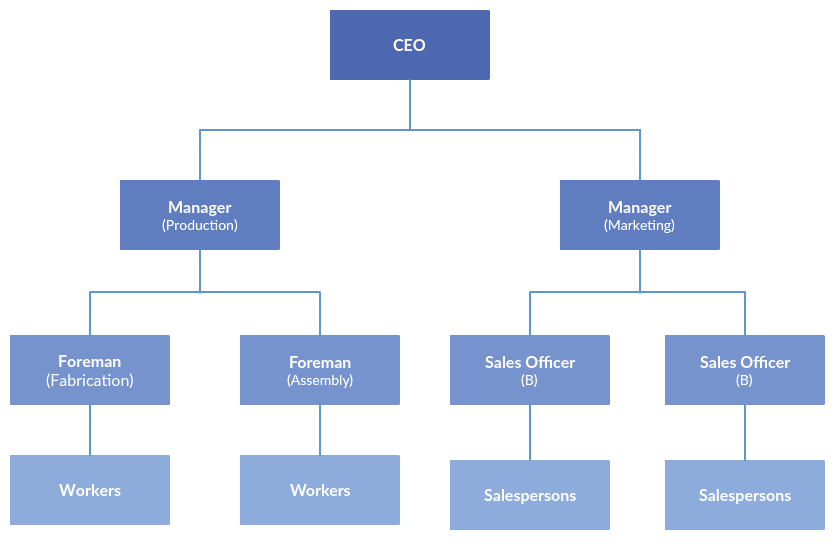
\includegraphics[scale=0.45]{gambar/struktur-organisasi.png}
  % Keterangan gambar yang diinputkan
  \caption{Struktur Organisasi PT. NASA}
  % Label referensi dari gambar yang diinputkan
	\label{fig:strukturOrganisasi}
\end{figure}

% Contoh penggunaan referensi dari gambar yang diinputkan
Seperti yang bisa dilihat pada \ref{fig:strukturOrganisasi}, \lipsum[1]
\vspace{0.5ex}

  \cleardoublepage

  % Bab 3 tunjauan pustaka
	\chapter{TINJAUAN PUSTAKA}
\vspace{4ex}

\setlength{\parindent}{7ex}

\section{Roket Luar Angkasa}
\vspace{1ex}

\begin{figure} [!ht] \centering
	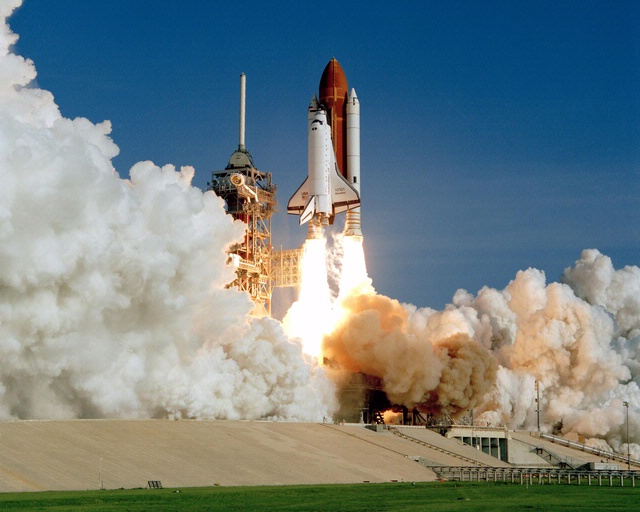
\includegraphics[scale=0.45]{gambar/space-shuttle.jpg}
	\caption{Peluncuran Pesawat Luar Angkasa \emph{Discovery}}
	\label{fig:spaceShuttle}
\end{figure}

Roket luar angkasa merupakan \lipsum[1]
\vspace{0.5ex}

\emph{Discovery} \ref{fig:spaceShuttle} merupakan \lipsum[2]

Beberapa keunggulan dari \lipsum[3][1-2] adalah:
\vspace{0.5ex}

\begin{enumerate}[nolistsep]

  \item Mempermudah \lipsum[1][1-2]
  \vspace{0.5ex}

  \item \lipsum[1][3-4]
  \vspace{0.5ex}

\end{enumerate}
\vspace{0.5ex}

\section{Gravitasi}
\vspace{1ex}

Gravitasi merupakan \lipsum[1]
\vspace{0.5ex}

\subsection{Hukum Newton}
\vspace{1ex}

Newton pernah merumuskan \citep{newtonLaw} bahwa \lipsum[2]
Kemudian menjadi persamaan seperti pada persamaan \ref{eq:hukumPertama}.
\vspace{0.5ex}

\begin{equation}\label{eq:hukumPertama}
  \sum \mathbf{F} = 0\; \Leftrightarrow\; \frac{\mathrm{d} \mathbf{v} }{\mathrm{d}t} = 0.
\end{equation}
\vspace{0.5ex}

\subsection{Anti Gravitasi}
\vspace{1ex}

Anti gravitasi sendiri merupakan \lipsum[3]
\vspace{0.5ex}
  \cleardoublepage

  % Bab 4 desain dan implementasi
	\chapter{DESAIN DAN IMPLEMENTASI}
\vspace{4ex}

\setlength{\parindent}{7ex}

\section{Deskripsi Sistem}
\vspace{1ex}

Sistem akan dibuat dengan \lipsum[1]
\vspace{0.5ex}

\lipsum[2]
\vspace{0.5ex}

\newpage

\section{Implementasi Alat}
\vspace{1ex}

Alat diimplementasikan dengan \lipsum[3]
\vspace{0.5ex}

\lstinputlisting[
  language=Python,
  label={lst:bilanganPrima},
  caption={Perhitungan Bilangan Prima}
]{program/prime-number.py}
\vspace{0.5ex}

Seperti contoh pada baris program \ref{lst:bilanganPrima} \lipsum[4]
\vspace{0.5ex}
  \cleardoublepage

  % Bab 5 pengujian dan evaluasi
	\chapter{PENGUJIAN DAN EVALUASI}
\vspace{4ex}

\setlength{\parindent}{7ex}

\section{Skenario Pengujian}
\vspace{1ex}

Pengujian dilakukan dengan \lipsum[1]
\vspace{0.5ex}

\lipsum[2]
\vspace{0.5ex}

\newpage

\section{Evaluasi Pengujian}
\vspace{1ex}

Dari pengujian yang \lipsum[3]
\vspace{0.5ex}

Sesuai dengan hasil pada \ref{tb:energiKecepatan} didapatkan \lipsum[4]

\begin{longtable}{|l|l|}
	\caption{Hasil Pengukuran Energi dan Kecepatan}
	\vspace{1.5ex}
	\label{tb:energiKecepatan}\\
	\hline
	\rowcolor[HTML]{C0C0C0}
	\textbf{Energi} & \textbf{Kecepatan} \\ \hline
	10 J & 200 m/s \\ \hline
	20 J & 400 m/s \\ \hline
	30 J & 800 m/s \\ \hline
	40 J & 1600 m/s \\ \hline
\end{longtable}
\vspace{1ex}

\lipsum[5]
\vspace{0.5ex}
  \cleardoublepage

  % Bab 6 kesimpulan dan saran
	% Ubah kalimat sesuai dengan judul dari bab ini
\chapter{KESIMPULAN DAN SARAN}
\vspace{4ex}

% Pengaturan ukuran indentasi
\setlength{\parindent}{7ex}

% Ubah konten-konten berikut sesuai dengan yang ingin diisi pada bab ini

\section{Kesimpulan}
\vspace{1ex}

Kesimpulan yang kami peroleh dari \lipsum[1][1] adalah:
\vspace{0.5ex}

\begin{enumerate}[nolistsep]

  \item Pembuatan \lipsum[1][1-2]
  \vspace{0.5ex}

  \item \lipsum[1][3-4]
  \vspace{0.5ex}

  \item \lipsum[1][5-6]
  \vspace{0.5ex}

\end{enumerate}
\vspace{0.5ex}

\section{Saran}
\vspace{1ex}

Saran yang kami ajukan dalam \lipsum[1][1] antara lain:
\vspace{0.5ex}

\begin{enumerate}[nolistsep]

  \item Sebaiknya \lipsum[1][1-2]
  \vspace{0.5ex}

  \item \lipsum[1][3-4]
  \vspace{0.5ex}

  \item \lipsum[1][5-6]
  \vspace{0.5ex}

\end{enumerate}
\vspace{0.5ex}
  \cleardoublepage

  % Daftar pustaka
  \renewcommand\bibname{DAFTAR PUSTAKA}
  \addcontentsline{toc}{chapter}{\bibname}
  \titlespacing*{\chapter}{0pt}{0ex}{5ex}
  \appendix
  \bibliographystyle{apalike}
  \bibliography{pustaka/pustaka.bib}
  \cleardoublepage

\end{document}